\documentclass[10pt]{beamer}
\usetheme{metropolis}

% ── Packages ──
\usepackage{amsmath,amssymb,amsthm}
\usepackage{tikz}
\usetikzlibrary{positioning,arrows.meta}
\usepackage{graphicx}
\usepackage{array}

% ── Theorem environments ──
\theoremstyle{definition}
\newtheorem{defi}{Definition}[section]
\newtheorem{prop}{Proposition}[section]
\newtheorem{cor}{Corollary}[section]

\setbeamercolor{block title}{bg=red!75!black,fg=white}
\setbeamercolor{block body}{bg=yellow!10!white}

% ── Emoji definitions ──
\newcommand{\bean}{
\includegraphics[scale=0.07]{Pictures/bean.png}}
\newcommand{\leaf}{
\includegraphics[scale=0.08]{Pictures/leaf.png}}
\newcommand{\lemon}{
\includegraphics[scale=0.08]{Pictures/lemon.png}}
\newcommand{\cow}{
\includegraphics[scale=0.08]{Pictures/cow.png}}
\newcommand{\milk}{
\includegraphics[scale=0.07]{Pictures/milk.png}}
\newcommand{\coffee}{
\includegraphics[scale=0.10]{Pictures/coffee.png}}
\newcommand{\tea}{
\includegraphics[scale=0.08]{Pictures/tea.png}}
\newcommand{\bento}{
\includegraphics[scale=0.09]{Pictures/bento.png}}
\newcommand{\ramen}{
\includegraphics[scale=0.09]{Pictures/soup.png}}

% ── Cross-filling color commands ──
\newcommand{\pvt}[1]{{\color{red}\mathbf{#1}}}       % pivot
\newcommand{\crs}[1]{{\color{blue}#1}}                % cross arm
\newcommand{\rem}[1]{{\color{gray}#1}}                % remainder zero

% ── Highlighting ──
\newcommand{\x}[1]{\alert{\textbf{#1}}}

\title{Cross-Filling Method}
\subtitle{Finding Hidden Patterns in Recipe Tables}
\date{}

\begin{document}

\maketitle

% ═══════════════════════════════════════
% §0 INTRODUCTION
% ═══════════════════════════════════════
\section{Introduction}

\begin{frame}{Learning Objectives}
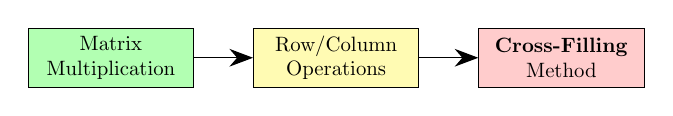
\begin{tikzpicture}[scale=0.75,transform shape,
    block/.style={draw, rectangle, minimum width=2.8cm, minimum height=1cm, align=center}]
\node[block,fill=green!30] (block1) {Matrix\\Multiplication};
\node[block, right=1cm of block1, fill=yellow!30] (block2) {Row/Column\\Operations};
\node[block, right=1cm of block2, fill=red!20] (block3) {\textbf{Cross-Filling}\\Method};
\draw[-{Stealth[length=3mm]}] (block1) -- (block2);
\draw[-{Stealth[length=3mm]}] (block2) -- (block3);
\end{tikzpicture}

\vspace{0.5cm}
\textbf{Key Questions:}
\begin{itemize}
\item Can we \x{discover hidden intermediate products} from a direct recipe table?
\item What is a \x{simple pattern} (rank-one table)?
\item How to \x{decompose} complex tables into simple patterns?
\item How to convert between \x{sum} and \x{product} forms?
\end{itemize}
\end{frame}

\begin{frame}{Review: Sum-of-Rank-One View}
Recall from Lecture 1, matrix multiplication $C = AB$ has three views:

$$C =
\begin{pmatrix}
| & | & & | \\
a_1 & a_2 & \cdots & a_n \\
| & | & & |
\end{pmatrix}
\begin{pmatrix}
- & b_1^T & - \\
- & b_2^T & - \\
\vdots & \vdots & \vdots \\
- & b_n^T & -
\end{pmatrix}
= \sum_{k=1}^{n} a_k \, b_k^T$$

\vfill
Each $a_k \, b_k^T$ is called a \x{rank-one piece} (column $\times$ row).

\vfill
\textbf{Today's question}: Can we \x{reverse} this? Given $C$, find the pieces?
\end{frame}

% ═══════════════════════════════════════
% §1 CONCRETIZATION PHASE: DISCOVERING PATTERNS
% ═══════════════════════════════════════
\section{Discovering Simple Patterns (Concretization)}

\begin{frame}{The Motivating Problem}
\textbf{Coffee shop scenario:}

We have a \x{direct} recipe table from raw materials to final products:
$$C = \begin{array}{c|cc}
 & \text{\bento} & \text{\ramen} \\
\hline
\text{\leaf} & 2 & 2 \\
\text{\lemon} & 1 & 1 \\
\text{\bean} & 0 & 4 \\
\text{\cow} & 2 & 1
\end{array}$$

\vfill
\textbf{Question}: Are there \x{hidden intermediate products} (like \milk, \coffee, \tea) that we could use to simplify this?
\end{frame}

\begin{frame}{What is a Simple Pattern?}
Look at the first two rows of our table:
$$\begin{array}{c|cc}
 & \text{\bento} & \text{\ramen} \\
\hline
\text{\leaf} & 2 & 2 \\
\text{\lemon} & 1 & 1
\end{array}$$

\vfill
\textbf{Notice}: Both products use \x{the same amount}!
\begin{itemize}
\item \bento: 2\leaf~+ 1\lemon
\item \ramen: 2\leaf~+ 1\lemon
\end{itemize}

\vfill
Can we extract this \x{common base} and see what's different?
\end{frame}

\begin{frame}{Setup: The Full Direct Table}
$$C = \begin{array}{c|cc}
 & \text{\bento} & \text{\ramen} \\
\hline
\text{\leaf} & 2 & 2 \\
\text{\lemon} & 1 & 1 \\
\text{\bean} & 0 & 4 \\
\text{\cow} & 2 & 1
\end{array}$$

\vfill
We noticed: first two rows have the same pattern.

\vfill
Can we \x{extract} this pattern and see what's left?
\end{frame}

\begin{frame}{Change: Choose a Pivot}
\textbf{Pick a pivot} (center of our cross):

Let's pick the \leaf~row and \bento~column. Entry = 2.

$$C = \begin{array}{c|cc}
 & \text{\bento} & \text{\ramen} \\
\hline
\text{\leaf} & \pvt{2} & 2 \\
\text{\lemon} & 1 & 1 \\
\text{\bean} & 0 & 4 \\
\text{\cow} & 2 & 1
\end{array}$$

\vfill
This pivot will be the \x{center of our cross}.
\end{frame}

\begin{frame}{Calculation Step 1: Extract the Cross}
The \x{cross} through the pivot includes:
\begin{itemize}
\item Entire \leaf~row (row through pivot)
\item Entire \bento~column (column through pivot)
\end{itemize}

$$C = \begin{array}{c|cc}
 & \text{\bento} & \text{\ramen} \\
\hline
\text{\leaf} & \pvt{2} & \crs{2} \\
\text{\lemon} & \crs{1} & 1 \\
\text{\bean} & \crs{0} & 4 \\
\text{\cow} & \crs{2} & 1
\end{array}$$

\vfill
Cross row: $(2, 2)$ \quad Cross column: $(2, 1, 0, 2)$
\end{frame}

\begin{frame}{Calculation Step 2: Build the Pattern Table}
\textbf{Idea}: Use the cross to fill all entries via "multiplication table":

$$\text{New entry} = \frac{\text{(column value)} \times \text{(row value)}}{\text{pivot}}$$

\vfill
For \ramen~and \lemon:
$$\text{Entry} = \frac{\crs{1} \times \crs{2}}{\pvt{2}} = 1$$

For \ramen~and \bean:
$$\text{Entry} = \frac{\crs{0} \times \crs{2}}{\pvt{2}} = 0$$
\end{frame}

\begin{frame}{Result: The First Pattern $R_1$}
$$R_1 = \begin{array}{c|cc}
 & \text{\bento} & \text{\ramen} \\
\hline
\text{\leaf} & \pvt{2} & \crs{2} \\
\text{\lemon} & \crs{1} & 1 \\
\text{\bean} & \crs{0} & 0 \\
\text{\cow} & \crs{2} & 2
\end{array}$$

\vfill
\textbf{Interpretation}: This is the \x{common base recipe}!
\begin{itemize}
\item Base recipe: 2\leaf~+ 1\lemon~+ 0\bean~+ 2\cow
\item \bento~uses: 1× base
\item \ramen~uses: 1× base (+ adjustments)
\end{itemize}
\end{frame}

\begin{frame}{Insight: What is This Pattern?}
The pattern $R_1$ is a \x{rank-one matrix}:

$$R_1 = \begin{pmatrix} 2 \\ 1 \\ 0 \\ 2 \end{pmatrix}
\begin{pmatrix} 1 & 1 \end{pmatrix}$$

\vspace{0.3cm}
- \x{Column} $(2,1,0,2)$: the base recipe
- \x{Row} $(1,1)$: both products use 1× this base

\vspace{0.3cm}
Key: \x{One pattern, repeated!} Both columns are the same.
\end{frame}

\begin{frame}{Setup: What's Left After $R_1$?}
Subtract $R_1$ from the original table $C$:

$$C - R_1 = \begin{array}{c|cc}
 & \text{\bento} & \text{\ramen} \\
\hline
\text{\leaf} & 2-2 & 2-2 \\
\text{\lemon} & 1-1 & 1-1 \\
\text{\bean} & 0-0 & 4-0 \\
\text{\cow} & 2-2 & 1-2
\end{array}$$
\end{frame}

\begin{frame}{Result: The Remainder}
$$C_2 = C - R_1 = \begin{array}{c|cc}
 & \text{\bento} & \text{\ramen} \\
\hline
\text{\leaf} & \rem{0} & \rem{0} \\
\text{\lemon} & \rem{0} & \rem{0} \\
\text{\bean} & \rem{0} & 4 \\
\text{\cow} & \rem{0} & -1
\end{array}$$

\vfill
\textbf{What's left?}
- \bento~column: all zeros (base recipe exactly matches!)
- \ramen~column: adjustments needed (+4\bean, -1\cow)
\end{frame}

\begin{frame}{Insight: Why "Cross-Filling"?}
\begin{center}
\begin{tikzpicture}[scale=0.6, every node/.style={scale=0.85}]
% Original
\node at (0,3) {\small Original};
\node at (0,1.5) {$\begin{array}{c|cc}
\text{\leaf} & 2 & 2 \\
\text{\lemon} & 1 & 1 \\
\text{\bean} & 0 & 4 \\
\text{\cow} & 2 & 1
\end{array}$};

% Arrow
\draw[-{Stealth},thick] (1.8,1.5) -- (3,1.5);
\node at (2.4,2) {\tiny pick pivot};

% Cross
\node at (5,3) {\small Extract \x{cross}};
\node at (5,1.5) {$\begin{array}{c|cc}
\text{\leaf} & \pvt{2} & \crs{2} \\
\text{\lemon} & \crs{1} & \cdot \\
\text{\bean} & \crs{0} & \cdot \\
\text{\cow} & \crs{2} & \cdot
\end{array}$};

% Arrow
\draw[-{Stealth},thick] (6.8,1.5) -- (8,1.5);
\node at (7.4,2) {\tiny fill};

% Filled
\node at (10,3) {\small \x{Fill} pattern};
\node at (10,1.5) {$\begin{array}{c|cc}
\text{\leaf} & \pvt{2} & \crs{2} \\
\text{\lemon} & \crs{1} & 1 \\
\text{\bean} & \crs{0} & 0 \\
\text{\cow} & \crs{2} & 2
\end{array}$};

% Arrow
\draw[-{Stealth},thick] (11.8,1.5) -- (13,1.5);
\node at (12.4,2) {\tiny subtract};

% Remainder
\node at (15,3) {\small Remainder};
\node at (15,1.5) {$\begin{array}{c|cc}
\text{\leaf} & \rem{0} & \rem{0} \\
\text{\lemon} & \rem{0} & \rem{0} \\
\text{\bean} & \rem{0} & 4 \\
\text{\cow} & \rem{0} & -1
\end{array}$};
\end{tikzpicture}
\end{center}

\vfill
The method \x{fills in} the cross region, then eliminates it!
\end{frame}

\begin{frame}{Change: Find Second Pattern}
Look at the remainder:
$$C_2 = \begin{array}{c|cc}
 & \text{\bento} & \text{\ramen} \\
\hline
\text{\bean} & 0 & 4 \\
\text{\cow} & 0 & -1
\end{array}$$

\vfill
This is the \x{adjustment} for \ramen: +4\bean, -1\cow

\vfill
Pick pivot: \bean~row, \ramen~column. Entry = 4.
\end{frame}

\begin{frame}{Calculation: Fill Second Cross}
Pivot at (3,2) = 4. Cross: column $(0,0,4,-1)^T$, row $(0,4)$

$$R_2 = \frac{1}{\pvt{4}}
\begin{pmatrix} 0 \\ 0 \\ 4 \\ -1 \end{pmatrix}
\begin{pmatrix} 0 & 4 \end{pmatrix}
= \begin{array}{c|cc}
 & \text{\bento} & \text{\ramen} \\
\hline
\text{\leaf} & 0 & 0 \\
\text{\lemon} & 0 & 0 \\
\text{\bean} & 0 & \pvt{4} \\
\text{\cow} & 0 & -1
\end{array}$$

\vfill
\textbf{Interpretation}: The \x{adjustment term} — only affects \ramen.
\end{frame}

\begin{frame}{Result: Complete Decomposition}
$$C_2 - R_2 = \begin{array}{c|cc}
 & \text{\bento} & \text{\ramen} \\
\hline
\text{\bean} & 0 & 0 \\
\text{\cow} & 0 & 0
\end{array}$$

\vfill
\x{Done!} Remainder is zero.
\end{frame}

\begin{frame}{The Full Decomposition}
\textbf{We discovered:}
$$C = R_1 + R_2$$

$$\begin{array}{c|cc}
\text{\leaf} & 2 & 2 \\
\text{\lemon} & 1 & 1 \\
\text{\bean} & 0 & 4 \\
\text{\cow} & 2 & 1
\end{array}
=
\begin{array}{c|cc}
\text{\leaf} & 2 & 2 \\
\text{\lemon} & 1 & 1 \\
\text{\bean} & 0 & 0 \\
\text{\cow} & 2 & 2
\end{array}
+
\begin{array}{c|cc}
\text{\leaf} & 0 & 0 \\
\text{\lemon} & 0 & 0 \\
\text{\bean} & 0 & 4 \\
\text{\cow} & 0 & -1
\end{array}$$

\vfill
Two \x{rank-one patterns}: base recipe + adjustment!
\end{frame}

\begin{frame}{Insight: Base + Adjustment Decomposition}
\textbf{What we found:}

$$\text{\ramen} = 1 \times (\text{base recipe}) + \text{adjustment}$$

\vfill
Key insight:
\begin{itemize}
\item $R_1$: Common base shared by both products
\item $R_2$: Adjustment term (only for \ramen)
\item \bento~= exactly the base recipe
\item \ramen~= base + extra 4\bean~- 1\cow
\end{itemize}

\vfill
This is \x{expressing complex recipes in terms of simpler patterns}!
\end{frame}

% ═══════════════════════════════════════
% §2 CHANGE OF PERSPECTIVE
% ═══════════════════════════════════════
\section{Change of Perspective}

\begin{frame}{Change of Perspective}
\textbf{What we've learned so far:}
\begin{itemize}
\item \x{What} a simple pattern (rank-one) looks like — one base mix used in different amounts
\item \x{How} to extract patterns using cross-filling — pick pivot, fill cross, subtract
\item \x{Why} this works — discovers hidden intermediate products
\end{itemize}

\vspace{0.5cm}
\begin{alertblock}{From This Point Forward}
We \x{forget about coffee shops} and work with \x{abstract matrices}:
\begin{itemize}
\item \textbf{What}: Matrices $A$, $B$, $C$, rank-one pieces $R_k$
\item \textbf{How}: Cross-filling algorithm, sum $\leftrightarrow$ product conversion
\item \textbf{Why}: Compute rank, factorizations, solve equations
\end{itemize}
\end{alertblock}

\vspace{0.3cm}
This simplifies notation while preserving the intuition.
\end{frame}

% ═══════════════════════════════════════
% §3 FORMALIZATION PHASE: DEFINITIONS AND ALGORITHMS
% ═══════════════════════════════════════
\section{Rank-One Matrices (Formalization)}

\begin{frame}{Definition: Rank-One Matrix}
\begin{defi}[Rank-One Matrix]
A matrix $R$ is \x{rank-one} if it can be written as
$$R = \mathbf{u}\, \mathbf{v}^T$$
for some nonzero column vector $\mathbf{u}$ and nonzero row vector $\mathbf{v}^T$.
\end{defi}

\vspace{0.3cm}
Example:
$$R = \begin{pmatrix} 2 \\ 1 \\ 3 \end{pmatrix} \begin{pmatrix} 1 & 2 \end{pmatrix}
= \begin{pmatrix}
2 & 4 \\
1 & 2 \\
3 & 6
\end{pmatrix}$$

\vspace{0.2cm}
Key: All columns are multiples of $\mathbf{u}$. All rows are multiples of $\mathbf{v}^T$.
\end{frame}

\begin{frame}{Recognizing Rank-One Structure}
Is this matrix rank-one?
$$\begin{pmatrix}
6 & 9 & 3 \\
4 & 6 & 2 \\
10 & 15 & 5
\end{pmatrix}$$

\vfill
Check rows:
\begin{itemize}
\item Row 1: $(6, 9, 3) = 3 \cdot (2, 3, 1)$
\item Row 2: $(4, 6, 2) = 2 \cdot (2, 3, 1)$
\item Row 3: $(10, 15, 5) = 5 \cdot (2, 3, 1)$
\end{itemize}

\vfill
Yes!\ \ $R = \begin{pmatrix} 3 \\ 2 \\ 5 \end{pmatrix} \begin{pmatrix} 2 & 3 & 1 \end{pmatrix}$
\end{frame}

\begin{frame}{Cross-Product Property}
In a rank-one matrix $R = \mathbf{u}\,\mathbf{v}^T$, every entry is $r_{ij} = u_i v_j$.

\vfill
For any four entries forming a rectangle:
$$\boxed{r_{ij} \cdot r_{k\ell} = r_{i\ell} \cdot r_{kj}}$$

\vfill
\textbf{Why?}\ \ $(u_i v_j)(u_k v_\ell) = (u_i v_\ell)(u_k v_j) = u_i u_k v_j v_\ell$

\vfill
Check: In $\begin{pmatrix} 6 & 9 \\ 4 & 6 \end{pmatrix}$: \quad $6 \times 6 = 36 = 9 \times 4$ \quad $\checkmark$
\end{frame}

\begin{frame}{Not Every Matrix is Rank-One}
$$C = \begin{pmatrix}
2 & 4 \\
1 & 2 \\
3 & 7
\end{pmatrix}$$

\vfill
Check ratios: $\frac{4}{2} = 2$, \quad $\frac{2}{1} = 2$, \quad $\frac{7}{3} \neq 2$ \quad $\leftarrow$ Different!

\vfill
This is \x{not rank-one}. But can we write it as a \x{sum} of rank-one pieces?

$$C = \underbrace{\begin{pmatrix} ? \end{pmatrix}}_{R_1} + \underbrace{\begin{pmatrix} ? \end{pmatrix}}_{R_2} + \cdots$$

Cross-filling answers this!
\end{frame}

% ═══════════════════════════════════════
% §4 CROSS-FILLING ALGORITHM
% ═══════════════════════════════════════
\section{Cross-Filling Algorithm}

\begin{frame}{The Cross-Filling Algorithm}
\begin{prop}[Cross-Filling Algorithm]
\textbf{Input}: Matrix $A$ ($m \times n$)

\textbf{Output}: $A = R_1 + R_2 + \cdots + R_r$ (sum of rank-one matrices)

\textbf{Procedure}:
\begin{enumerate}
\item Find any nonzero entry $a_{ij} \neq 0$ (the \x{pivot})
\item Extract the cross: row $i$ and column $j$
\item Form rank-one piece:
$$R = \frac{1}{a_{ij}} \cdot (\text{column } j) \cdot (\text{row } i)$$
\item Compute remainder: $A' = A - R$
\item Repeat on $A'$ until $A' = O$
\end{enumerate}
\end{prop}

\vfill
Each step eliminates one cross (one row and one column become zero).
\end{frame}

\begin{frame}{Example: Cross-Filling a $3 \times 3$ Matrix}
Decompose:
$$A = \begin{pmatrix}
1 & 1 & 1 \\
1 & 3 & 3 \\
1 & 3 & 8
\end{pmatrix}$$

\vfill
We will peel off rank-one pieces iteratively.
\end{frame}

\begin{frame}{Iteration 1: Pivot $a_{11} = 1$}
Highlight the cross:
$$A = \begin{pmatrix}
\pvt{1} & \crs{1} & \crs{1} \\
\crs{1} & 3 & 3 \\
\crs{1} & 3 & 8
\end{pmatrix}$$

\vfill
Fill using the cross:
$$R_1 = \frac{1}{\pvt{1}}
\begin{pmatrix} \crs{1} \\ \crs{1} \\ \crs{1} \end{pmatrix}
\begin{pmatrix} \crs{1} & \crs{1} & \crs{1} \end{pmatrix}
= \begin{pmatrix}
\pvt{1} & \crs{1} & \crs{1} \\
\crs{1} & 1 & 1 \\
\crs{1} & 1 & 1
\end{pmatrix}$$
\end{frame}

\begin{frame}{Iteration 1: Remainder $A_1$}
$$A_1 = A - R_1 = \begin{pmatrix}
1 & 1 & 1 \\
1 & 3 & 3 \\
1 & 3 & 8
\end{pmatrix}
- \begin{pmatrix}
1 & 1 & 1 \\
1 & 1 & 1 \\
1 & 1 & 1
\end{pmatrix}
= \begin{pmatrix}
\rem{0} & \rem{0} & \rem{0} \\
\rem{0} & 2 & 2 \\
\rem{0} & 2 & 7
\end{pmatrix}$$

\vfill
Row 1 and column 1 are now \rem{zero}.\ \ $\checkmark$
\end{frame}

\begin{frame}{Iteration 2: Pivot $(A_1)_{22} = 2$}
$$A_1 = \begin{pmatrix}
\rem{0} & \rem{0} & \rem{0} \\
\rem{0} & \pvt{2} & \crs{2} \\
\rem{0} & \crs{2} & 7
\end{pmatrix}$$

\vfill
Fill:
$$R_2 = \frac{1}{\pvt{2}}
\begin{pmatrix} \rem{0} \\ \crs{2} \\ \crs{2} \end{pmatrix}
\begin{pmatrix} \rem{0} & \crs{2} & \crs{2} \end{pmatrix}
= \begin{pmatrix}
\rem{0} & \rem{0} & \rem{0} \\
\rem{0} & \pvt{2} & \crs{2} \\
\rem{0} & \crs{2} & 2
\end{pmatrix}$$
\end{frame}

\begin{frame}{Iteration 2: Remainder $A_2$}
$$A_2 = A_1 - R_2 = \begin{pmatrix}
0 & 0 & 0 \\
0 & 2 & 2 \\
0 & 2 & 7
\end{pmatrix}
- \begin{pmatrix}
0 & 0 & 0 \\
0 & 2 & 2 \\
0 & 2 & 2
\end{pmatrix}
= \begin{pmatrix}
\rem{0} & \rem{0} & \rem{0} \\
\rem{0} & \rem{0} & \rem{0} \\
\rem{0} & \rem{0} & 5
\end{pmatrix}$$

\vfill
Rows 1--2 and columns 1--2 are now \rem{zero}.\ \ $\checkmark$
\end{frame}

\begin{frame}{Iteration 3: Final Piece}
$$A_2 = \begin{pmatrix}
\rem{0} & \rem{0} & \rem{0} \\
\rem{0} & \rem{0} & \rem{0} \\
\rem{0} & \rem{0} & \pvt{5}
\end{pmatrix}$$

\vfill
This is already rank-one:
$$R_3 = \begin{pmatrix} 0 \\ 0 \\ 1 \end{pmatrix}
\begin{pmatrix} 0 & 0 & 5 \end{pmatrix}
= \begin{pmatrix}
\rem{0} & \rem{0} & \rem{0} \\
\rem{0} & \rem{0} & \rem{0} \\
\rem{0} & \rem{0} & \pvt{5}
\end{pmatrix}$$

Remainder: $A_3 = A_2 - R_3 = O$. \quad \x{Done!}
\end{frame}

\begin{frame}{Full Decomposition}
$$A = \underbrace{\begin{pmatrix}
\pvt{1} & \crs{1} & \crs{1} \\
\crs{1} & 1 & 1 \\
\crs{1} & 1 & 1
\end{pmatrix}}_{R_1}
+ \underbrace{\begin{pmatrix}
\rem{0} & \rem{0} & \rem{0} \\
\rem{0} & \pvt{2} & \crs{2} \\
\rem{0} & \crs{2} & 2
\end{pmatrix}}_{R_2}
+ \underbrace{\begin{pmatrix}
\rem{0} & \rem{0} & \rem{0} \\
\rem{0} & \rem{0} & \rem{0} \\
\rem{0} & \rem{0} & \pvt{5}
\end{pmatrix}}_{R_3}$$

\vfill
Three rank-one pieces:
\begin{itemize}
\item $R_1$: pivot $\pvt{1}$ at position $(1,1)$
\item $R_2$: pivot $\pvt{2}$ at position $(2,2)$
\item $R_3$: pivot $\pvt{5}$ at position $(3,3)$
\end{itemize}
\end{frame}

\begin{frame}{Definition: Rank of a Matrix}
\begin{defi}[Rank]
The \x{rank} of a matrix $A$ is the number of rank-one pieces in its cross-filling decomposition:
$$A = R_1 + R_2 + \cdots + R_r \quad \Longrightarrow \quad \operatorname{rank}(A) = r$$
\end{defi}

\vspace{0.3cm}
\textbf{Examples:}
\begin{itemize}
\item Zero matrix $O$: rank $0$
\item Rank-one matrix $\mathbf{u}\mathbf{v}^T$: rank $1$
\item Identity $I_n$: rank $n$
\item Our $A$ above: rank $3$
\end{itemize}

\vspace{0.2cm}
\textbf{Important}: Different pivot choices give different decompositions, but always the same count $r$. (Proved in Lecture 4.)
\end{frame}

% ═══════════════════════════════════════
% §5 SUM ↔ PRODUCT EQUIVALENCE
% ═══════════════════════════════════════
\section{Sum $\leftrightarrow$ Product Equivalence}

\begin{frame}{From Sum to Product Form}
Each rank-one piece is an \x{outer product}:
$$R_k = \mathbf{u}_k \, \mathbf{v}_k^T$$

\vfill
From our example:
\begin{align*}
R_1 &= \begin{pmatrix} 1 \\ 1 \\ 1 \end{pmatrix}
\begin{pmatrix} 1 & 1 & 1 \end{pmatrix} \\[6pt]
R_2 &= \begin{pmatrix} 0 \\ 1 \\ 1 \end{pmatrix}
\begin{pmatrix} 0 & 2 & 2 \end{pmatrix} \\[6pt]
R_3 &= \begin{pmatrix} 0 \\ 0 \\ 1 \end{pmatrix}
\begin{pmatrix} 0 & 0 & 5 \end{pmatrix}
\end{align*}
\end{frame}

\begin{frame}{Collecting the Pieces}
Collect columns $\mathbf{u}_k$ into $U$, rows $\mathbf{v}_k^T$ into $V$:
$$U = \begin{pmatrix}
| & | & | \\
\mathbf{u}_1 & \mathbf{u}_2 & \mathbf{u}_3 \\
| & | & |
\end{pmatrix}
= \begin{pmatrix}
1 & 0 & 0 \\
1 & 1 & 0 \\
1 & 1 & 1
\end{pmatrix}$$

$$V = \begin{pmatrix}
- & \mathbf{v}_1^T & - \\
- & \mathbf{v}_2^T & - \\
- & \mathbf{v}_3^T & -
\end{pmatrix}
= \begin{pmatrix}
1 & 1 & 1 \\
0 & 2 & 2 \\
0 & 0 & 5
\end{pmatrix}$$

By sum-of-rank-one:\ \ $UV = \sum_{k=1}^{3} \mathbf{u}_k\, \mathbf{v}_k^T = R_1 + R_2 + R_3 = A$
\end{frame}

\begin{frame}{Verification}
$$UV = \begin{pmatrix}
1 & 0 & 0 \\
1 & 1 & 0 \\
1 & 1 & 1
\end{pmatrix}
\begin{pmatrix}
1 & 1 & 1 \\
0 & 2 & 2 \\
0 & 0 & 5
\end{pmatrix}
= \begin{pmatrix}
1 & 1 & 1 \\
1 & 3 & 3 \\
1 & 3 & 8
\end{pmatrix} = A \quad \checkmark$$

\vfill
Notice: $U$ is \x{lower triangular}, $V$ is \x{upper triangular}!

\vfill
This happened because we chose \x{diagonal pivots} $(1,1) \to (2,2) \to (3,3)$.

\vfill
Key: Diagonal pivots $\Longrightarrow$ \x{LU decomposition} (preview of future lecture).
\end{frame}

\begin{frame}{Sum $\leftrightarrow$ Product Equivalence}
\begin{prop}[Sum $\leftrightarrow$ Product]
For any matrix $A$:
$$A = \sum_{k=1}^r \mathbf{u}_k\,\mathbf{v}_k^T \quad \Longleftrightarrow \quad A = U \cdot V$$
where $U$ has columns $\mathbf{u}_k$ and $V$ has rows $\mathbf{v}_k^T$.
\end{prop}

\vfill
Two directions:
\begin{itemize}
\item \textbf{Lecture 1}: Given product $A = UV$, read off sum $A = \sum \mathbf{u}_k\,\mathbf{v}_k^T$
\item \textbf{Today}: Given sum from cross-filling, assemble product $A = UV$
\end{itemize}
\end{frame}

\begin{frame}{The Inner Dimension}
When $A = UV$ with $A$ being $m \times n$:
$$A_{m \times n} = U_{m \times \boxed{r}} \cdot V_{\boxed{r} \times n}$$

The shared dimension $r$ is the \x{inner dimension}.

\vfill
\begin{itemize}
\item Outer dimensions $m, n$: visible (size of $A$)
\item Inner dimension $r$: \x{hidden} = number of independent patterns
\end{itemize}

\vfill
Key: $\operatorname{rank}(A) = r$ = inner dimension of the factorization.
\end{frame}

% ═══════════════════════════════════════
% §6 ALGEBRAIC FORMULA
% ═══════════════════════════════════════
\section{Algebraic Expression for Cross-Filling}

\begin{frame}{Cross-Filling as a Matrix Formula}
Let $e_i$ be the $i$-th column of $I$, and $e_j^T$ the $j$-th row of $I$.

\vfill
Then:
\begin{itemize}
\item $Ae_i$ = column $i$ of $A$
\item $e_j^T A$ = row $j$ of $A$
\item $e_j^T A e_i$ = entry $(j,i)$ of $A$ = the pivot
\end{itemize}

\vfill
The cross-filling formula at pivot position (row $j$, column $i$):
$$\boxed{R = A e_i \, (e_j^T A e_i)^{-1} \, e_j^T A}$$

\vfill
This is: $\dfrac{1}{\text{pivot}} \times \text{(column)} \times \text{(row)}$
\end{frame}

\begin{frame}{Example Verification}
$A = \begin{pmatrix} 1 & 1 & 1 \\ 1 & 3 & 3 \\ 1 & 3 & 8 \end{pmatrix}$, \quad cross-fill at row 1, column 1:

\vfill
\begin{align*}
Ae_1 &= \begin{pmatrix} 1 \\ 1 \\ 1 \end{pmatrix}, \quad
e_1^T A = \begin{pmatrix} 1 & 1 & 1 \end{pmatrix}, \quad
e_1^T A e_1 = 1
\end{align*}

$$R_1 = \begin{pmatrix} 1 \\ 1 \\ 1 \end{pmatrix} \cdot 1 \cdot \begin{pmatrix} 1 & 1 & 1 \end{pmatrix}
= \begin{pmatrix}
1 & 1 & 1 \\
1 & 1 & 1 \\
1 & 1 & 1
\end{pmatrix} \quad \checkmark$$
\end{frame}

\begin{frame}{Application: Projection Matrices}
\begin{defi}[Projection]
A square matrix $P$ is a \x{projection} if $P^2 = P$.
\end{defi}

\vfill
\begin{prop}
If $P$ is a projection and $R$ is obtained by cross-filling from $P$, then $R$ is also a projection.
\end{prop}

\vfill
\textbf{Proof}: Let $R = Pe_i(e_j^TPe_i)^{-1}e_j^TP$. Then
\begin{align*}
R^2 &= Pe_i(e_j^TPe_i)^{-1} \underbrace{e_j^T P \cdot P e_i}_{= \, e_j^TPe_i} (e_j^TPe_i)^{-1}e_j^TP \\
&= Pe_i(e_j^TPe_i)^{-1}e_j^TP = R \quad \checkmark
\end{align*}

(Used $P^2 = P$ in the underbraced step.)
\end{frame}

\begin{frame}{Projection Decomposition}
If $P$ is a projection and $R$ comes from cross-filling $P$:
$$P = \underbrace{R}_{\text{projection}} + \underbrace{(P-R)}_{\text{also projection!}}$$

\vspace{0.3cm}
Check: $(P-R)^2 = P^2 + R^2 - PR - RP = P + R - R - R = P - R$ \quad $\checkmark$

\vspace{0.3cm}
Cross-filling \x{decomposes projections into smaller projections}.

This will be \x{crucial} for spectral decomposition (future lecture).
\end{frame}

% ═══════════════════════════════════════
% §7 PREVIEW: LU DECOMPOSITION
% ═══════════════════════════════════════
\section{Preview: LU Decomposition}

\begin{frame}{Preview: Diagonal Pivots $\Rightarrow$ LU}
In our example, diagonal pivots produced:
$$A = \underbrace{\begin{pmatrix}
1 & 0 & 0 \\
1 & 1 & 0 \\
1 & 1 & 1
\end{pmatrix}}_{\text{lower triangular } L}
\underbrace{\begin{pmatrix}
1 & 1 & 1 \\
0 & 2 & 2 \\
0 & 0 & 5
\end{pmatrix}}_{\text{upper triangular } U}$$

\vfill
Key: The pivots $\pvt{1}, \pvt{2}, \pvt{5}$ appear on the diagonal of $U$.

\vfill
Diagonal cross-filling $\Longrightarrow$ \x{LU decomposition}.

\vfill
\begin{alertblock}{Preview (Future Lecture)}
LU decomposition is a special case of cross-filling with diagonal pivot strategy.
Full theory, including PLU decomposition, will be covered in Week 3.
\end{alertblock}
\end{frame}

\begin{frame}{Not All Matrices Have Diagonal LU}
Diagonal cross-filling requires \x{nonzero diagonal pivots}. But this can fail:

$$A = \begin{pmatrix} 0 & 3 \\ 1 & 2 \end{pmatrix}$$

Pivot $a_{11} = 0$ — cannot start!

\vspace{0.3cm}
Even later pivots can fail:
$$\begin{pmatrix} 1 & 2 & 3 \\ 1 & 2 & 4 \\ 1 & 3 & 5 \end{pmatrix}
\xrightarrow{\text{after } R_1} \begin{pmatrix}
\rem{0} & \rem{0} & \rem{0} \\
\rem{0} & \pvt{0} & 1 \\
\rem{0} & 1 & 2
\end{pmatrix}$$

Second pivot is $\pvt{0}$!

\vspace{0.2cm}
\textbf{Solution}: Allow non-diagonal pivots, or permute rows first $\to$ \x{PLU} (future lecture).
\end{frame}

% ═══════════════════════════════════════
% §8 SUMMARY
% ═══════════════════════════════════════
\section{Summary}

\begin{frame}{Summary}
\textbf{Today we learned:}

\begin{enumerate}
\item \textbf{Rank-one matrix}: $R = \mathbf{u}\,\mathbf{v}^T$ (one pattern, repeated)

\item \textbf{Cross-filling algorithm}: Decompose any matrix into rank-one pieces
$$A = R_1 + R_2 + \cdots + R_r$$
Pick pivot → Extract cross → Fill → Subtract → Repeat

\item \textbf{Sum $\leftrightarrow$ Product equivalence}:
$$\sum_{k=1}^r \mathbf{u}_k\,\mathbf{v}_k^T = A = UV$$

\item \textbf{Rank} = number of pieces = inner dimension of $UV$

\item \textbf{Algebraic formula}: $R = Ae_i(e_j^TAe_i)^{-1}e_j^TA$

\item \textbf{Applications}: Projection decomposition, preview of LU decomposition
\end{enumerate}
\end{frame}

\begin{frame}{Looking Ahead}
\textbf{Lecture 4} (next week):
\begin{itemize}
\item \x{Well-definedness of rank} — Why does rank not depend on pivot choices?
\item \x{Linear independence} and \x{basis} — Two languages for subspaces
\item \x{Dimension} — Connection to rank via trace
\item Solving $Ax = b$ using cross-filling
\end{itemize}

\vfill
\textbf{The big picture}:
\begin{center}
Cross-filling $\to$ Rank $\to$ Subspaces $\to$ Projections $\to$ Spectral Decomposition
\end{center}

Every major topic connects back to rank-one decomposition!
\end{frame}

\end{document}
